\section{Calibration en énergie des jets dans CMS}\label{chapter-JERC-section-CMS}
Les jets sont des objets physiques composites complexes qu'il est nécessaire de calibrer, comme tout autre objet reconstruit.
La précision apportée à la mesure des jets est capitale dans de nombreuses analyses, où il s'agit d'une source majeure d'incertitude systématique.
Les avancées réalisées récemment sur la calibration des jets ont ainsi permis d'améliorer la précision sur la mesure de la section efficace inclusive de production de jets et de la masse du quark top~\cite{JERC_RunI}.
\par À partir des jets reconstruits par les méthodes décrites précédemment, un procédé de correction de l'énergie des jets (JEC, \emph{Jet Energy Correction}) est réalisé.
Il permet de corriger l'échelle en énergie des jets (JES, \emph{Jet Energy Scale}) ainsi que la résolution sur cette énergie (JER, \emph{Jet Energy Resolution}).
La collaboration CMS utilise une approche factorisée dans laquelle plusieurs étapes corrigent chacune un effet en particulier et dépendent des étapes précédentes~\cite{JERC_RunI}.
La figure~\ref{fig-CMS-JME-13-004_Figure_002-TeX} résume ces étapes, décrites dans les sections qui suivent.
\begin{figure}[h]
\centering
\includegraphics[width=\textwidth]{\PhDthesisdir/plots_and_images/from_JERC_RunI/CMS-JME-13-004_Figure_002-FR-TeX.tex}
\caption[Étapes successives de la JEC.]{Étapes successives de la JEC pour les données et les simulations~\cite{JERC_RunI}. Les corrections des étapes marquées \og MC \fg{} sont obtenues par l'étude de simulations, celles marquées \og RC \fg{} par une méthode de cône aléatoire (\emph{Random Cone}) sur les données. Les types d'événements utilisés dans les corrections résiduelles sont également indiqués.}
\label{fig-CMS-JME-13-004_Figure_002-TeX}
\end{figure}
\par Trois stades ou \og niveaux \fg{} de correction sur les particules peuvent être définis.
\begin{itemize}
\item Le niveau \og particule \fg, noté \ptcl, ou niveau \og vrai \fg{}, se réfère aux objets et variables après hadronisation mais avant interaction avec le détecteur. Il s'agit donc des grandeurs recherchées, uniquement accessibles dans les événements simulés.
\item Le niveau \og reconstruit \fg, noté \reco, correspond aux objets et variables après interaction avec le détecteur et reconstruction par l'algorithme de \PF.
\item Le niveau \og corrigé \fg{} ou calibré, noté \cali, correspond aux objets et variables corrigés, \ie\ ceux du niveau reconstruit auxquels ont été appliquées les corrections.
\end{itemize}
La réponse d'un jet, variable importante pour ce chapitre, est définie comme
\begin{equation}
R = \frac{\pT}{\pT_\ptcl}
\mend
\label{eq-def_R_jet}
\end{equation}
La réponse peut être définie à différents niveaux, et par définition $R_\ptcl=1$.
Si la JEC est correcte, alors l'impulsion transverse du jet corrigé doit correspondre sensiblement à l'impulsion transverse au niveau particule, \ie\ $R_\cali\simeq1$.
Sur la figure~\ref{fig-JERC_RunI-1} sont représentées les réponses de jets d'événements QCD simulés à différentes étapes de la JEC. Après avoir appliqué toutes les corrections, ce qui correspond à la figure~\ref{subfig-JERC_RunI-1_3}, la réponse est sensiblement égale à 1, ce qui montre que la JEC est correcte.
\begin{figure}[h]
\centering
\subcaptionbox{Avant correction ($R_\reco$).\label{subfig-JERC_RunI-1_1}}[.3\textwidth]
{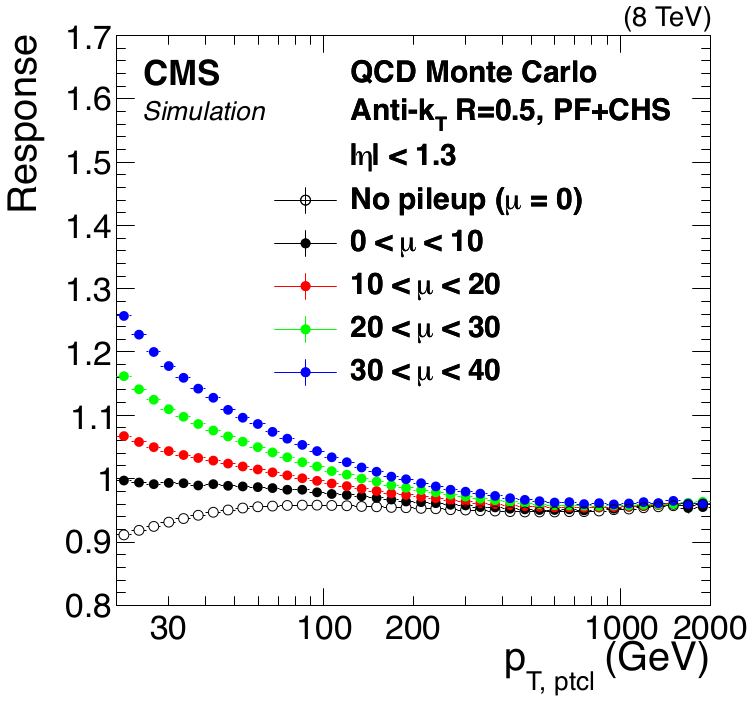
\includegraphics[width=.3\textwidth]{\PhDthesisdir/plots_and_images/from_JERC_RunI/response_evolution_1.png}}
\hfill
\subcaptionbox{Correction de l'empilement.\label{subfig-JERC_RunI-1_2}}[.3\textwidth]
{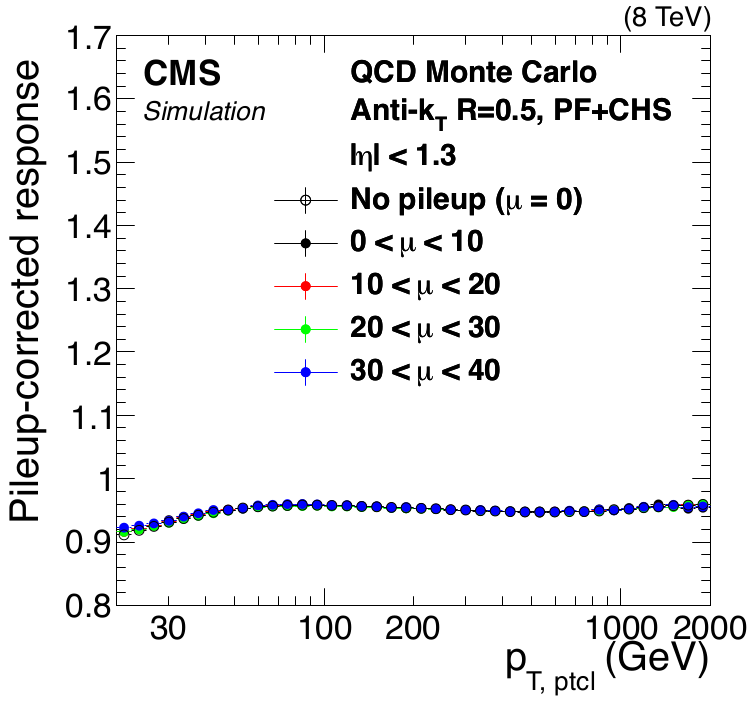
\includegraphics[width=.3\textwidth]{\PhDthesisdir/plots_and_images/from_JERC_RunI/response_evolution_2.png}}
\hfill
\subcaptionbox{Après correction ($R_\cali$).\label{subfig-JERC_RunI-1_3}}[.3\textwidth]
{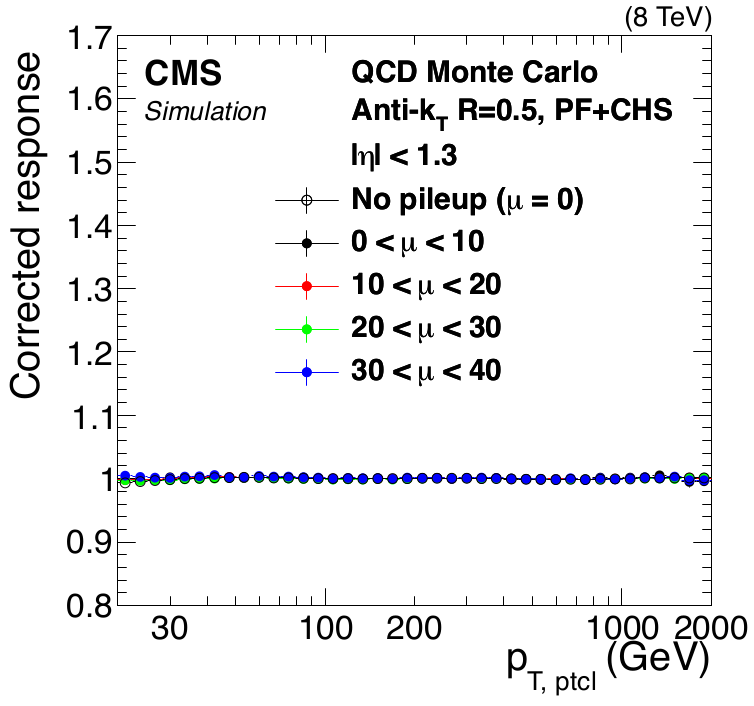
\includegraphics[width=.3\textwidth]{\PhDthesisdir/plots_and_images/from_JERC_RunI/response_evolution_3.png}}
\caption[Valeur moyenne de la réponse de jets d'événements QCD simulés.]{Valeur moyenne de la réponse de jets d'événements QCD simulés en fonction de $\pT_\ptcl$ à différentes étapes de la JEC~\cite{JERC_RunI} et pour différentes valeurs d'interactions d'empilement $\mu$.}
\label{fig-JERC_RunI-1}
\end{figure}
\par Les jets au niveau particule sont reconstruits en appliquant la procédure de recombinaison à toutes les particules de durée de vie $\tau$ telle que $c\tau>\SI{1}{\centi\meter}$ à l'exception des neutrinos~\cite{JERC_RunI}.
Les hadrons contenant des quarks~\quarkc\ ou~\quarkb\ ne rentrent pas dans cette catégorie et ce sont donc leurs produits de désintégration qui sont pris en compte pour la recombinaison.
Les neutrinos sont exclus pour pouvoir définir la réponse des jets d'une manière qui soit accessible expérimentalement et qui réduise significativement les différences de réponse entre jets lourds et jets légers ou de gluons, à cause des neutrinos produits dans les désintégration des quarks lourds.
\subsection{Correction de l'empilement}\label{chapter-JERC-section-CMS-subsec-PU}
Des contributions additionnelles à l'énergie et à l'impulsion des jets peuvent apparaître du fait de l'empilement, décrit dans la section~\ifref{chapter-LHC-section-LHC-subsec-PU}{\ref{chapter-LHC-section-LHC-subsec-PU}}{1.4} du chapitre~\ifref{chapter-LHC}{\ref{chapter-LHC}}{3}.
La correction de l'empilement a pour but de soustraire ces contributions et est appliquée dans les données et les événements simulés.
Elle permet d'améliorer la résolution en énergie des jets et d'obtenir une JES plus précise.
\par L'empilement asynchrone est réduit par l'analyse temporelle des signaux des calorimètres,
l'empilement synchrone par la méthode de soustraction des hadrons chargés (CHS, \emph{pile-up Charged Hadron Subtraction}), décrite ci-après.
\par Pour chacun des vertex primaires de l'événement, la somme des impulsions transverses au carré des traces associées au vertex est calculée.
Le vertex primaire principal est choisi comme étant le vertex présentant la plus grande valeur de cette somme.
Les autres vertex primaires sont considérés comme des vertex d'empilement.
Les hadrons chargés dont les traces associées proviennent de vertex d'empilement sont retirés de l'événement.
La reconstruction des jets est alors réalisée à partir de l'événement nettoyé, ce qui permet d'améliorer la résolution en \pT\ des jets.
\par La correction de l'empilement résiduel $\mathcal{C}_\text{PU}$, principalement due aux hadrons neutres, aux photons, aux traces non associées à un vertex et à l'empilement asynchrone qui n'a pas pu être corrigé totalement, s'exprime en fonction de
\begin{itemize}
\item l'impulsion transverse du jet avant application de cette correction et après CHS, $\pT_\reco^\text{CHS}$;
\item la pseudo-rapidité du jet, $\eta$;
\item l'aire du jet dans le plan $(\eta, \phi)$, $A$;
\item la densité en énergie dans le plan $(\eta, \phi)$ de l'événement contenant ce jet, notée $\rho$;
\end{itemize}
sous la forme
\begin{equation}
\mathcal{C}_\text{PU}(\pT_\reco^\text{CHS}, \eta, A, \rho)
= 1 - \frac{\average{\pT_\ptcl^\text{add}}}{\pT_\reco^\text{CHS}}
\label{eq-chapter-JERC-section-CMS-subsec-PU-offset_corr_v2}
\end{equation}
où $\average{\pT_\ptcl^\text{add}}$ est la contribution additionnelle de l'empilement au niveau particule, estimée à l'aide de la méthode de l'aire hybride (\emph{hybrid jet area}) à partir d'événements QCD multijet simulés avec et sans empilement, \ie
\begin{equation}
\average{\pT_\ptcl^\text{add}}(\rho, \eta, \pT_\reco^\text{CHS})
=
\average{\pT_\ptcl^\text{avec PU} - \pT_\ptcl^\text{sans PU}}
\mend[,]
\label{eq-chapter-JERC-section-CMS-subsec-PU-pTaddptcl}
\end{equation}
avec
$\pT_\ptcl^\text{avec PU}$ et $\pT_\ptcl^\text{sans PU}$
les impulsions du jet au niveau particule avec et sans empilement.
La contribution additionnelle de l'empilement au niveau particule est alors paramétrée en fonction de $\pT_\reco^\text{CHS}$, $\eta$, $A$ et $\rho$ et la correction de l'empilement résiduel $\mathcal{C}_\text{PU}$ définie par~\eqref{eq-chapter-JERC-section-CMS-subsec-PU-offset_corr_v2} peut se réécrire
\begin{equation}
\mathcal{C}_\text{PU}(\pT_\reco^\text{CHS}, \eta, A, \rho)
= 1 - \frac{\left[\rho_0(\eta) + \rho\,\beta(\eta)(1+\gamma(\eta)\log\pT_\reco^\text{CHS})\right]A}{\pT_\reco^\text{CHS}}
\label{eq-chapter-JERC-section-CMS-subsec-PU-offset_corr_v1}
\end{equation}
où $\rho_0(\eta)$, $\beta(\eta)$ et $\gamma(\eta)$ sont les paramètres de cette correction, dépendants de $\eta$.
\par La figure~\ref{fig-chapter-JERC-section-CMS-subsec-PU-JERC_RunI-Figure_005} montre $\average{\pT_\ptcl^\text{add}}$ en fonction de l'impulsion transverse du jet au niveau particule, avant et après application de la correction de l'empilement.
Les résultats de la figure~\ref{subfig-chapter-JERC-section-CMS-subsec-PU-JERC_RunI-Figure_005b} sont cohérents avec l'absence d'énergie supplémentaire due à l'empilement à $\pm\SI{0.2}{\GeV}$ jusqu'à $\pT_\ptcl = \SI{500}{\GeV}$ et à $\pm\SI{0.6}{\GeV}$ au-delà.
%Dans le cas d'un grand nombre d'interactions d'empilement ($\mu>30$), un léger effet est visible, lié à une dépendance quadratique en $\rho$ de la contribution en énergie de l'empilement qui n'est pas modélisée~\cite{JERC_RunI}.
\begin{figure}[h]
\centering
\subcaptionbox{Avant correction.\label{subfig-chapter-JERC-section-CMS-subsec-PU-JERC_RunI-Figure_005a}}[.45\textwidth]
{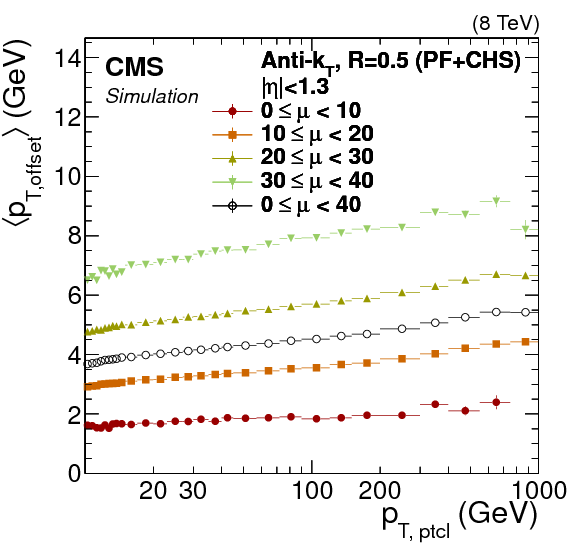
\includegraphics[width=.45\textwidth]{\PhDthesisdir/plots_and_images/from_JERC_RunI/Figure_005-a.tex}}
\hfill
\subcaptionbox{Après correction.\label{subfig-chapter-JERC-section-CMS-subsec-PU-JERC_RunI-Figure_005b}}[.45\textwidth]
{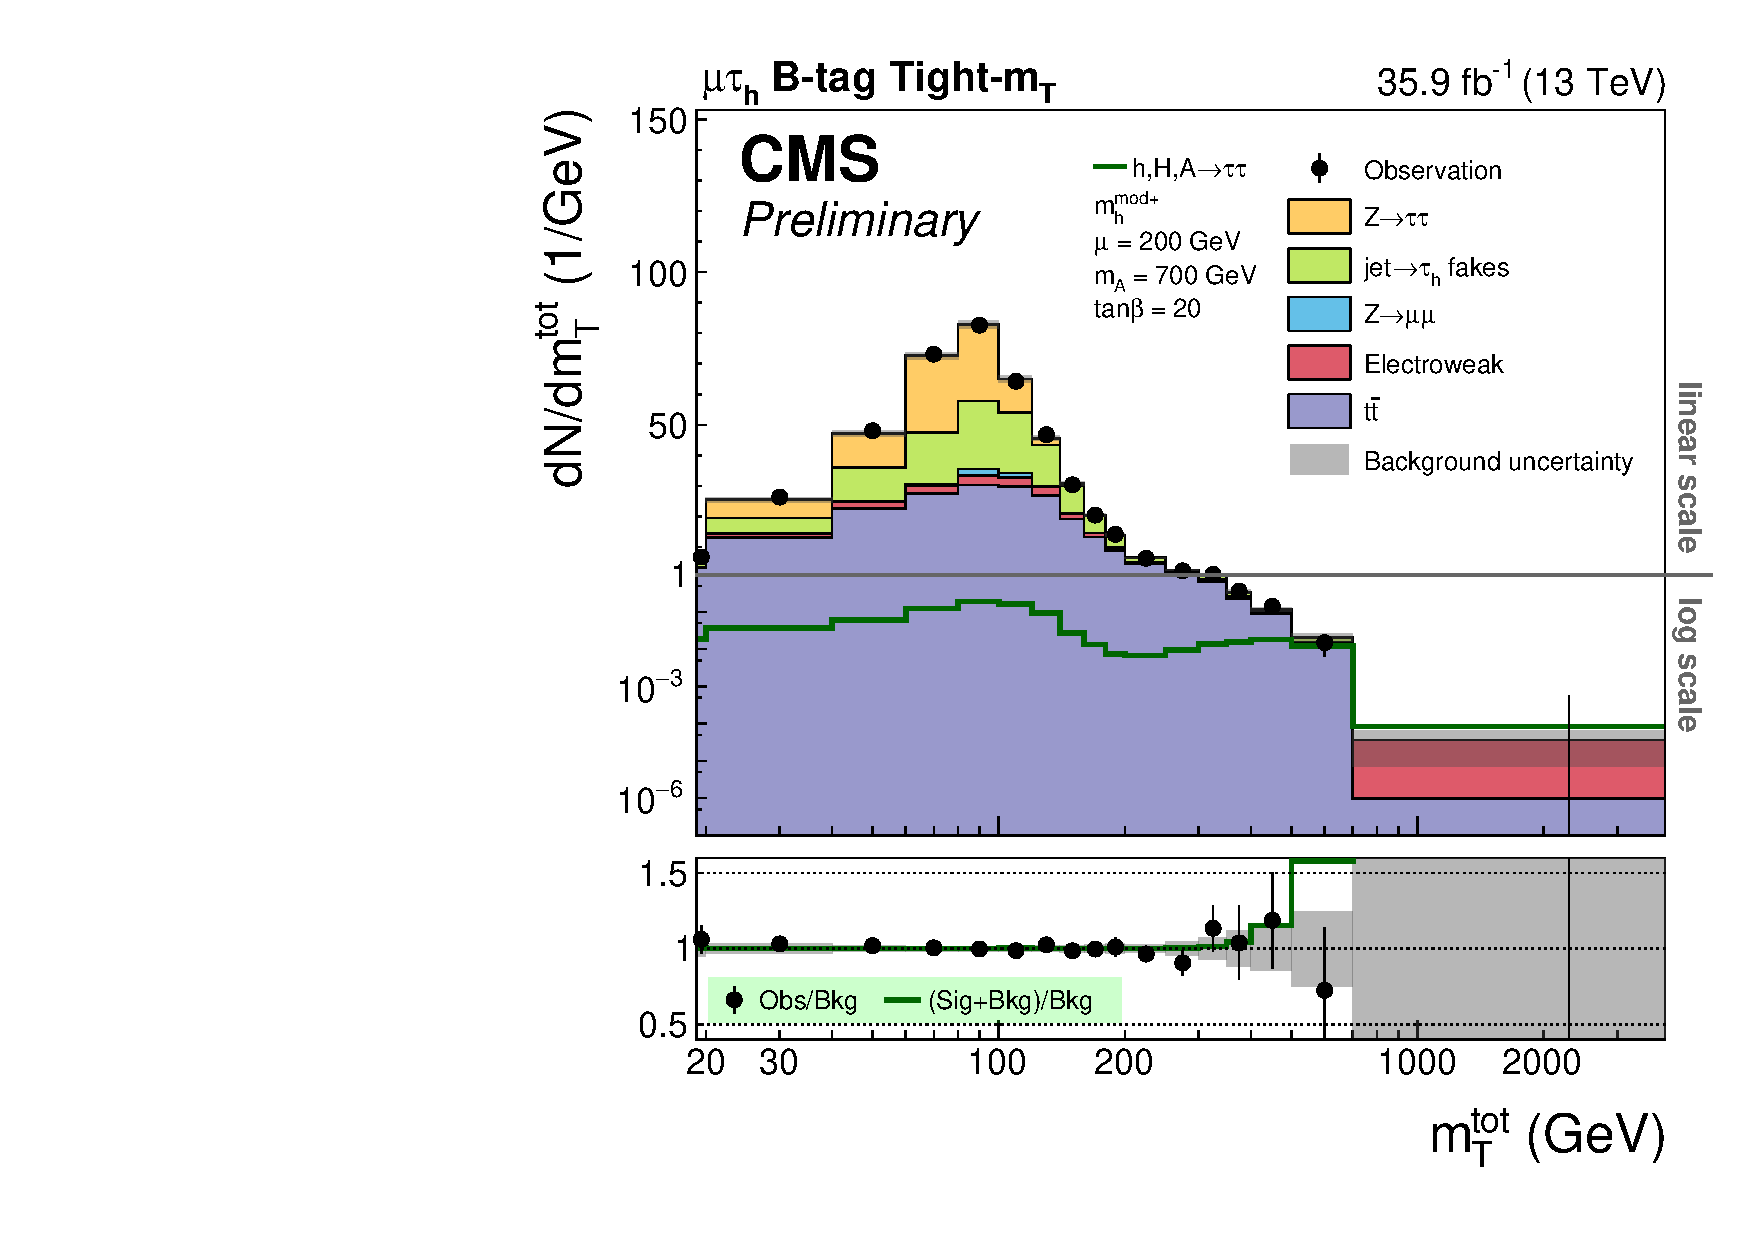
\includegraphics[width=.45\textwidth]{\PhDthesisdir/plots_and_images/from_JERC_RunI/Figure_005-b.tex}}
\caption[Contribution additionnelle de l'empilement au niveau particule.]{Contribution additionnelle de l'empilement au niveau particule telle que définie dans l'équation~\eqref{eq-chapter-JERC-section-CMS-subsec-PU-pTaddptcl} pour $\abs{\eta}<\num{1.3}$ en fonction de l'impulsion du jet au niveau particule pour différentes valeurs du nombre d'interaction d'empilement ($\mu$)~\cite{JERC_RunI}.}
\label{fig-chapter-JERC-section-CMS-subsec-PU-JERC_RunI-Figure_005}
\end{figure}
\par La correction ainsi décrite doit être légèrement adaptée pour pouvoir l'appliquer aux données à cause des biais de simulation du détecteur.
Pour cela, un ajustement en fonction de $\eta$ est déterminé à l'aide de la méthode de cône aléatoire (RC, \emph {Random Cone}). La méthode RC reconstruit les jets à l'aide de cônes dont la direction en $(\eta, \phi)$ est choisie de manière aléatoire.
L'étude est réalisée sur des événements dits de \og zéro biais \fg.
Il s'agit d'événements sélectionnés par un déclenchement aléatoire pendant que les faisceaux de protons se croisent.
Le déclenchement n'étant pas dû à un dépôt d'énergie en particulier, ces événements ne comportent pas, en général, de contribution provenant d'une interaction dure, \ie\ d'une collision effective entre les protons.
Dans ce cas, la valeur moyenne de l'impulsion transverse des jets reconstruits par la méthode RC permet d'estimer la moyenne de la contribution additionnelle de l'empilement, \ie
\begin{equation}
\average{\pT^\text{add}}^\text{RC} = \average{\pT_\text{cône}}
\mend
\end{equation}
Il est alors possible de définir un facteur d'échelle à appliquer aux paramètres $\rho_0$ et $\beta$ de l'équation~\eqref{eq-chapter-JERC-section-CMS-subsec-PU-offset_corr_v1} lorsque cette correction est appliquée aux données. Ce facteur d'échelle s'exprime
\begin{equation}
\frac{\average{\pT^\text{add}}^\text{RC}_\text{données}(\eta, \rho_\text{données})}{\average{\pT^\text{add}}^\text{RC}_\text{simulation}(\eta, \rho_\text{simulation})}
\mend
\end{equation}
La contribution additionnelle de l'empilement est ainsi corrigée dans les simulations et les données.
\subsection{Correction de la réponse du détecteur en $\pT$ et en $\eta$}\label{chapter-JERC-section-CMS-subsec-reponse}
La réponse du détecteur CMS à un jet n'est pas uniforme selon la valeur de \pT\ et $\eta$ du jet.
La réponse au niveau reconstruit de jets simulés $R_\reco$,
déterminée grâce à une simulation du détecteur CMS basée sur \GEANTfour~\cite{geant4_2003,geant4_2006,geant4_2016},
combinée à \PYTHIA~6.4~\cite{pythia6.4}
avec les réglages Z2*~\cite{tunes_2016},
est représentée sur la figure~\ref{fig-simulated_jet_response_RunII} pour les trois années du Run~II du LHC.
Il apparaît, par exemple, qu'un jet de $\pT=\SI{30}{\GeV}$ nécessite une correction allant de \SI{10}{\%} dans la région centrale $\abs{\eta}<\num{0.7}$ à plus de \SI{30}{\%} lorsque $\abs{\eta}\simeq\num{3}$ en 2017 et 2018.
\begin{figure}[h]
\centering
\subcaptionbox{Année 2016.\label{subfig-simulated_jet_response_2016}}[.3\textwidth]
{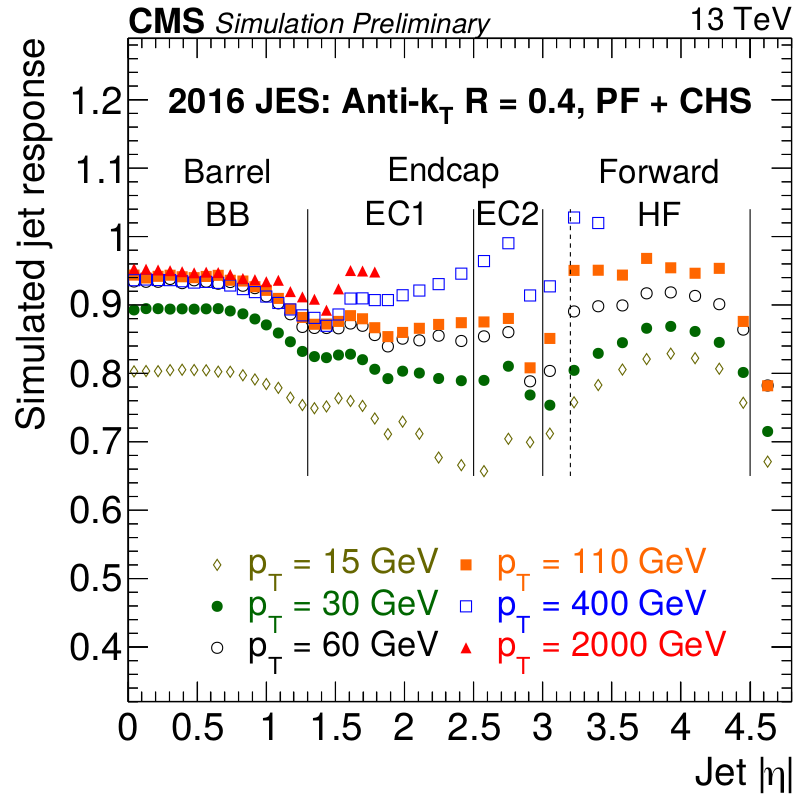
\includegraphics[width=.3\textwidth]{\PhDthesisdir/plots_and_images/from_CMS-DP-2020-019/simulated_jet_response_2016.png}}
\hfill
\subcaptionbox{Année 2017.\label{subfig-simulated_jet_response_2017}}[.3\textwidth]
{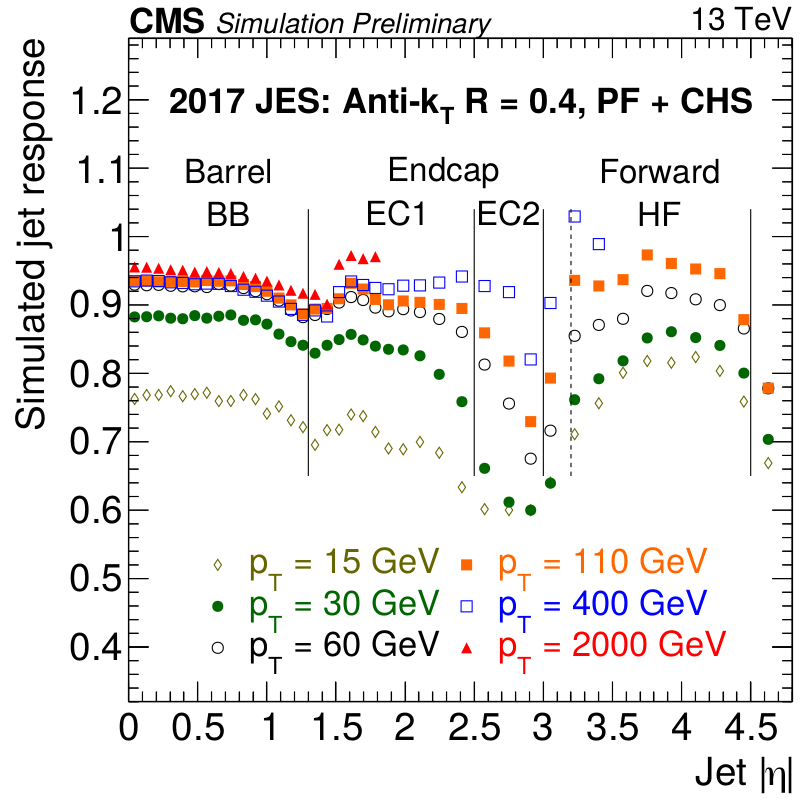
\includegraphics[width=.3\textwidth]{\PhDthesisdir/plots_and_images/from_CMS-DP-2020-019/simulated_jet_response_2017.png}}
\hfill
\subcaptionbox{Année 2018.\label{subfig-simulated_jet_response_2018}}[.3\textwidth]
{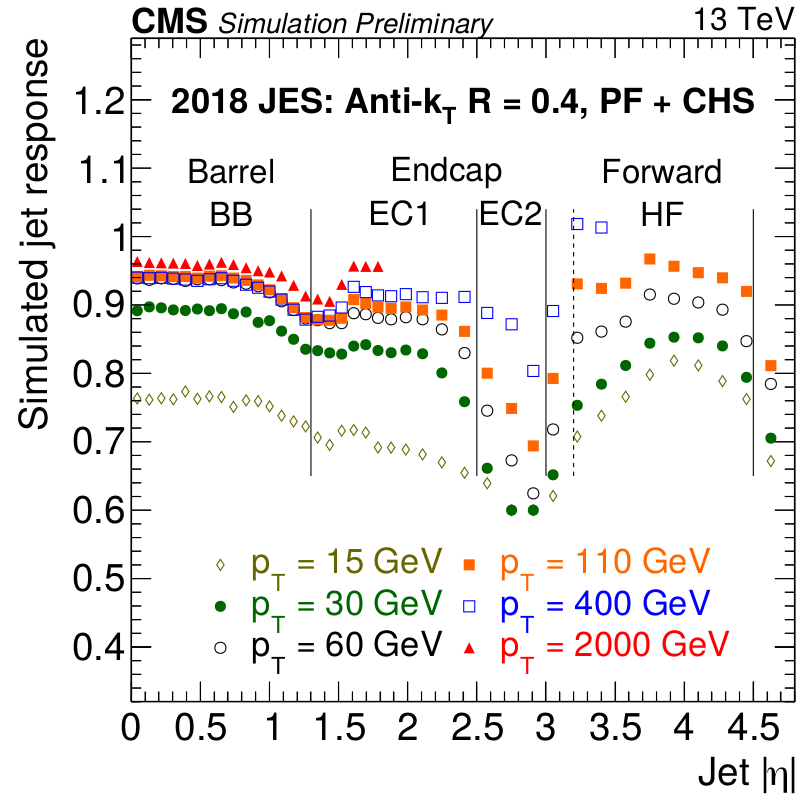
\includegraphics[width=.3\textwidth]{\PhDthesisdir/plots_and_images/from_CMS-DP-2020-019/simulated_jet_response_2018.png}}
\caption[Réponse des jets reconstruits en fonction de \pT\ et $\eta$ lors du Run~II.]{Réponse des jets reconstruits en fonction de \pT\ et $\eta$ lors du Run~II~\cite{CMS-DP-2020-019}. La chute de la réponse des jets dans la région $\abs{\eta}\simeq\num{3}$ est due à la transition entre le bouchon (\emph{Endcap}) et la partie avancée (\emph{Forward}) du détecteur. Pour $\abs{\eta}>\num{4.5}$, les limites du détecteur en termes d'acceptation expliquent la chute de la réponse des jets. La dégradation au cours du temps du détecteur dans la région \og EC2 \fg{} s'observe par la baisse de la réponse des jets dans cette région de 2016 à 2017.}
\label{fig-simulated_jet_response_RunII}
\end{figure}
\par Afin de corriger la réponse du détecteur en $\pT$ et en $\eta$, la correction $\mathcal{C}_\text{Rép}$ à appliquer s'exprime
\begin{equation}
\mathcal{C}_\text{Rép}(\pT_\reco', \eta) = \frac{\average{\pT_\ptcl}}{\average{\pT_\reco'}} = \frac{1}{\average{R_\reco'}}
\end{equation}
où $\pT_\reco'$ est l'impulsion transverse du jet après correction de l'empilement.
Les moyennes sont réalisées sur les jets appartenant à la même cellule d'une grille en $(\pT_\ptcl, \eta)$ prédéfinie~\cite{JERC_RunI}.
\subsection{Corrections résiduelles}\label{chapter-JERC-section-CMS-subsec-residuals}
Les corrections décrites dans les sections précédentes permettent d'obtenir une bonne correction en énergie des jets.
Toutefois, des différences dans les réponses des jets, de l'ordre du pourcent, subsistent entre données et simulations.
Des corrections résiduelles à appliquer aux données sont ainsi déterminées afin de réduire ces écarts, définies telles que
\begin{equation}
\mathcal{C}_\text{Res} = \frac{R_\text{simulations}}{R_\text{données}}
\mend
\label{eq-chapter-JERC-section-CMS-subsec-residuals-Cres_def}
\end{equation}
\par Le principe est d'estimer la réponse du jet en s'appuyant sur un objet de référence pouvant être un boson \Zboson\ (événements \Zjets), un photon (événements \Gjets) ou un autre jet (événements dijet et multijet).
Deux méthodes existent et sont utilisées de manière complémentaire:
\begin{description}
\item[la méthode de la balance] estime que l'objet de référence et le jet sont balancés au niveau particule, \ie\ d'impulsion transverse totale nulle, soit
\begin{equation}
\vpT_\ptcl^\text{réf} + \vpT_\ptcl^\text{jet} = \vec{0}
\mend
\label{eq-chapter-JERC-section-CMS-subsec-residuals-pT_bal_ppe1}
\end{equation}
L'objet de référence étant fidèlement reconstruit,
\begin{equation}
\vpT_\reco^\text{réf} \simeq \vpT_\ptcl^\text{réf} = \vpT^\text{réf}
\mend
\label{eq-chapter-JERC-section-CMS-subsec-residuals-pT_ref_approx_ptcl_reco}
\end{equation}
Ainsi, l'équation~\eqref{eq-chapter-JERC-section-CMS-subsec-residuals-pT_bal_ppe1} peut se réécrire à l'aide de~\eqref{eq-chapter-JERC-section-CMS-subsec-residuals-pT_ref_approx_ptcl_reco} sous la forme
\begin{equation}
\vpT^\text{réf} + \vpT_\ptcl^\text{jet} = \vec{0}
\mend
\label{eq-chapter-JERC-section-CMS-subsec-residuals-pT_bal_ppe2}
\end{equation}
La réponse d'un jet définie par~\eqref{eq-def_R_jet} permet alors de faire apparaître la réponse balancée du jet, notée \Rbal,
\begin{equation}
\vpT^\text{réf} + \frac{1}{\Rbal} \vpT_\reco^\text{jet} = \vec{0}
\mend
\label{eq-chapter-JERC-section-CMS-subsec-residuals-pT_bal_ppe3}
\end{equation}
Il en résulte
\begin{equation}
\Rbal (\pT, \eta) = \frac{\pT_\reco^\text{jet}}{\pT^\text{réf}}
\label{eq-chapter-JERC-section-CMS-subsec-residuals-Rbal_def}
\end{equation}
\item[la méthode \og MPF \fg] (\emph{MET Projection Fraction}) prend en compte l'ensemble de l'activité hadronique de l'événement et considère l'impulsion de recul vis-à-vis de l'objet de référence, \ie
\begin{equation}
\vpT_\ptcl^\text{réf} + \vpT_\ptcl^\text{recul} = \vec{0}
\mend
\label{eq-chapter-JERC-section-CMS-subsec-residuals-pT_MPF_ppe1}
\end{equation}
Au niveau reconstruit, l'impulsion transverse manquante (MET) définie dans la section~\ifref{chapter-LHC-section-evt_reco-subsec-MET}{\ref{chapter-LHC-section-evt_reco-subsec-MET}}{6.3} du chapitre~\ifref{chapter-LHC}{\ref{chapter-LHC}}{3} doit être prise en compte dans le recul.
Afin de garder une description cohérente de l'événement, les corrections précédentes apportées aux jets sont d'abord propagées à \vMET.
L'équation précédente, valable au niveau particule, s'écrit alors
\begin{equation}
\vpT_\reco^\text{réf} + \vpT_\reco^\text{recul} = -\vMET
\end{equation}
%Afin de garder une description cohérente de l'événement, les corrections apportées aux jets sont propagées à la MET par la correction dite de \og type-I \fg,
%\begin{equation}
%\vMET = \vMET_\text{type-I} = \vMET_\reco + \sum_{\substack{\text{jets}\\\pT_\reco>\SI{15}{\GeV}}} \left(\vpT_\reco - \vpT_\cali\right) - \vec{\mathcal{O}}_\text{RC}
%\end{equation}
%où $\vpT_\cali$ correspond à l'impulsion transverse du jet après application des corrections des étapes précédentes de la JEC
%et
%$\vec{\mathcal{O}}_\text{RC}$ la contribution moyenne de l'empilement obtenue par la méthode RC.
La réponse d'un jet définie par~\eqref{eq-def_R_jet} permet alors de faire apparaître la réponse MPF du jet, notée \RMPF,
\begin{equation}
\vpT_\reco^\text{réf} + \RMPF\vpT_\ptcl^\text{recul} = -\vMET
\mend
\end{equation}
En appliquant~\eqref{eq-chapter-JERC-section-CMS-subsec-residuals-pT_ref_approx_ptcl_reco} et~\eqref{eq-chapter-JERC-section-CMS-subsec-residuals-pT_MPF_ppe1} à l'équation précédente, il est possible d'écrire
\begin{equation}
\vpT^\text{réf} - \RMPF\vpT^\text{réf} = -\vMET
\mend
\end{equation}
Par produit scalaire avec $\vpT^\text{réf}$, il vient
\begin{equation}
\abs{\vpT^\text{réf}}^2 (1-\RMPF) = -\vpT^\text{réf}\cdot\vMET
\mend[,]
\end{equation}
ce qui permet de définir \RMPF\ comme
\begin{equation}
\RMPF (\pT, \eta) = 1 + \frac{\vpT^\text{réf}\cdot\vMET}{\abs{\vpT^\text{réf}}^2}
\mend
\end{equation}
\end{description}
\subsubsection{Correction résiduelle relative en $\eta$}\label{chapter-JERC-section-CMS-subsec-residuals_eta}
La première de ces corrections résiduelles, fonction de $\eta$, est obtenue à partir de la comparaison données-simulations sur une sélection d'événements dijet.
Son but est de rendre indépendant de $\eta$ le rapport données sur simulations de la réponse des jets.
Cette correction s'appuie sur la bonne reconstruction des jets dans le barillet.
Lorsqu'un événement présente un premier jet avec $\abs{\eta}<\num{1.3}$, \ie\ dans la région de référence du barillet, et un second avec $\abs{\eta}>\num{1.3}$ et de \pT\ similaire, le premier sert d'objet de référence afin de calibrer le second; c'est pourquoi cette correction est qualifiée de \og relative \fg.
La correction à appliquer aux données ainsi obtenue est illustrée sur la figure~\ref{fig-L2ResRel_RunII} dans le cas des jets d'impulsion transverse égale à \SI{120}{\GeV}.
\begin{figure}[h]
\centering
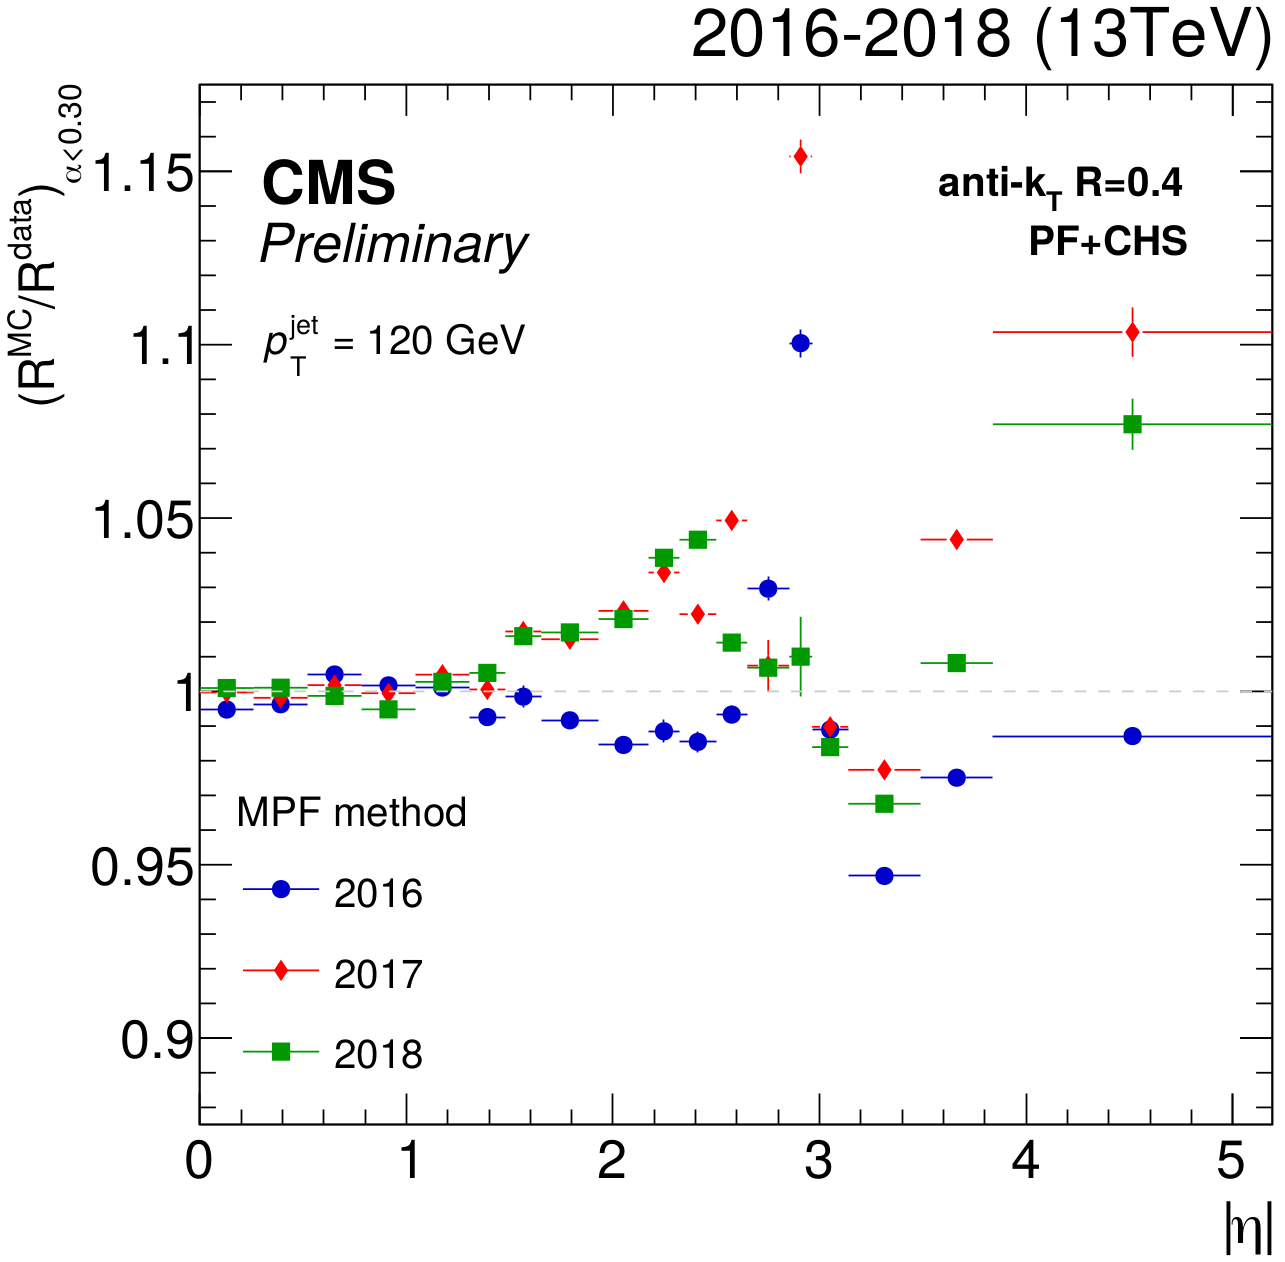
\includegraphics[width=.45\textwidth]{\PhDthesisdir/plots_and_images/from_CMS-DP-2020-019/relative_eta_residual_RunII.png}
\caption[Correction résiduelle relative en $\eta$ lors du Run~II.]{Correction résiduelle relative en $\eta$ lors du Run~II obtenue avec des événements dijet et la méthode MPF~\cite{CMS-DP-2020-019}.}
\label{fig-L2ResRel_RunII}
\end{figure}
\subsubsection{Correction résiduelle absolue en \pT}\label{chapter-JERC-section-CMS-subsec-residuals_pT}
Cette correction, fonction de \pT, a pour but de rendre indépendant de \pT\ le rapport données sur simulations de la réponse des jets.
Elle combine, à l'aide d'un ajustement global, les comparaisons données-simulations de plusieurs types d'événements afin de couvrir un large spectre de valeurs de \pT. Chaque type d'événement est en effet dominant, de par sa statistique, dans une gamme de \pT\ donnée:
\begin{itemize}
\item événements \Zjets: il s'agit d'événements \Zmmjets\ et \Zeejets, sélectionnés par la présence d'une paire de muons ou d'électrons compatibles avec la désintégration d'un \Zboson, ils couvrent la région $\pT<\SI{400}{\GeV}$;
\item événements \Gjets: sélectionnés dans les données à l'aide d'un déclenchement basé sur la présence d'un photon, ils permettent de traiter la région $\SI{100}{\GeV}<\pT<\SI{1000}{\GeV}$;
\item événements multijet: ces événements contiennent au moins deux jets dans l'état final et couvrent la région $\pT>\SI{200}{\GeV}$.
\end{itemize}
En 2017 et 2018, les événements multijet n'ont pas été exploités et la correction résiduelle absolue en \pT\ dans la région $\pT>\SI{800}{\GeV}$ est contrainte par l'analyse des événements \Gjets.
\par Cette correction corrige l'échelle en énergie absolue des jets, d'où son qualificatif, à partir d'un objet de référence pouvant être un boson \Zboson\ (\Zjets), un photon (\Gjets) ou un autre jet (multijet).
La correction à appliquer aux données ainsi obtenue est illustrée sur la figure~\ref{fig-L3ResAbs_RunII} dans le cas des jets de pseudo-rapidité $\abs{\eta}<\num{1.3}$.
\begin{figure}[h]
\centering
\subcaptionbox{Année 2016.\label{subfig-absolute_pT_residual_2016}}[.3\textwidth]
{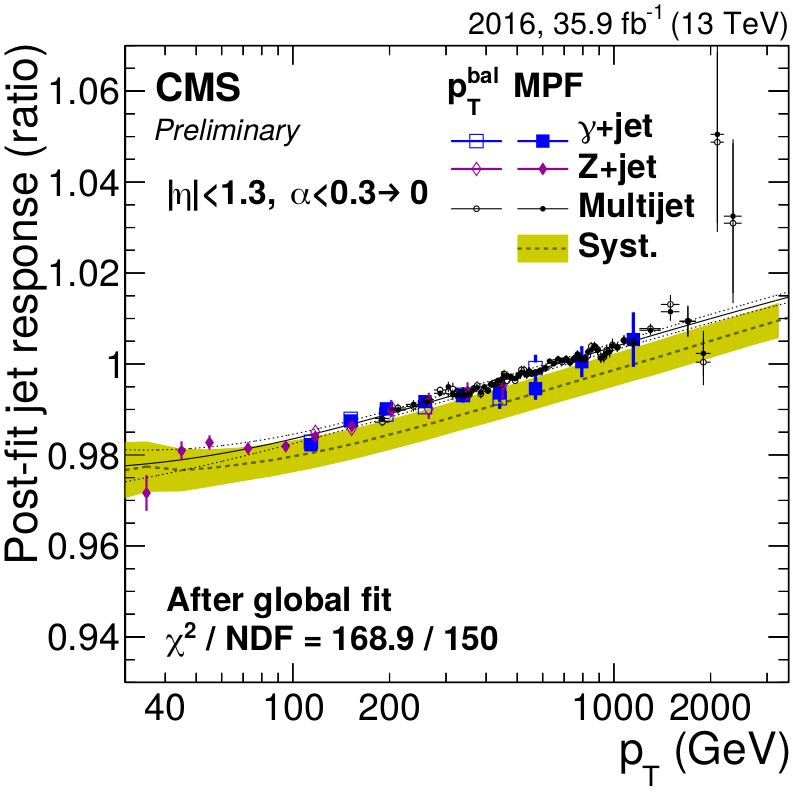
\includegraphics[width=.3\textwidth]{\PhDthesisdir/plots_and_images/from_CMS-DP-2020-019/absolute_pT_residual_2016.png}}
\hfill
\subcaptionbox{Année 2017.\label{subfig-absolute_pT_residual_2017}}[.3\textwidth]
{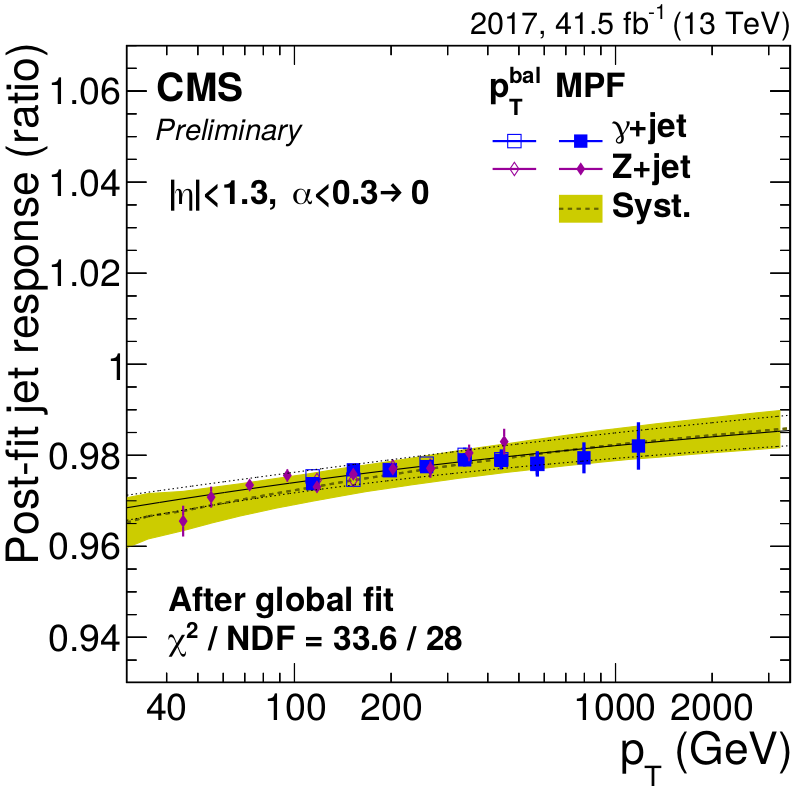
\includegraphics[width=.3\textwidth]{\PhDthesisdir/plots_and_images/from_CMS-DP-2020-019/absolute_pT_residual_2017.png}}
\hfill
\subcaptionbox{Année 2018.\label{subfig-absolute_pT_residual_2018}}[.3\textwidth]
{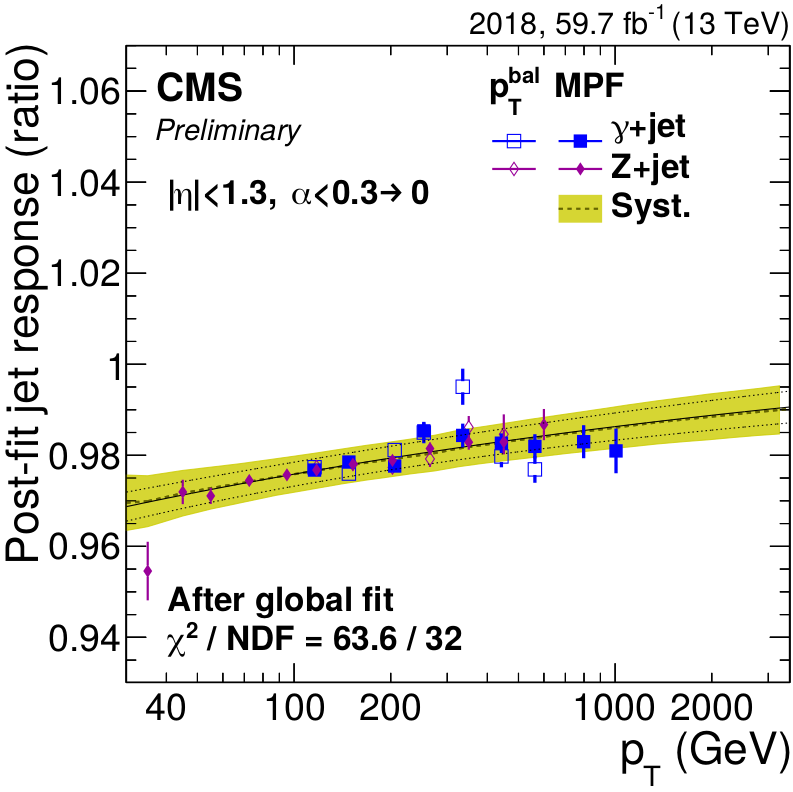
\includegraphics[width=.3\textwidth]{\PhDthesisdir/plots_and_images/from_CMS-DP-2020-019/absolute_pT_residual_2018.png}}
\caption[Correction résiduelle absolue en $\pT$ pour $\abs{\eta}<\num{1.3}$ lors du Run~II.]{Correction résiduelle absolue en $\pT$ pour $\abs{\eta}<\num{1.3}$ lors du Run~II obtenue par ajustement global sur les événements \Gjets, \Zjets\ et multijet~\cite{CMS-DP-2020-019}.}
%Mikko:
%We are now using multijet again, thanks to getting it back to Helsinki, reverting back closer to Run 1 method and actually pushing hard to understand and reduce the systematic uncertainties. And it’s working wonderfully! We’re for sure going to use multijet for all UL samples. Now is the first time it’s actually more constraining at high pT than gamma+jet.
\label{fig-L3ResAbs_RunII}
\end{figure}
\par Durant ma thèse, j'étais responsable de la mesure de cette correction avec les événements \Gjets\ pour les années 2018, utilisés dans la figure~\ref{subfig-absolute_pT_residual_2018} afin de réaliser un ajustement global avec les autres analyses, et 2017-UL.
La phénoménologie de ces événements ainsi que leur analyse sont détaillées dans les sections~\ref{chapter-JERC-section-pheno-GJets} et~\ref{chapter-JERC-section-JES}.
%une fois le ECAL calibré (test de presque chaque cristal en faisceau), calibration du HCAL.
\newpage
\subsubsection{Correction résiduelle de saveur}\label{chapter-JERC-section-CMS-subsec-residuals_flavor}
\begin{wrapfigure}{R}{8cm}
\centering
\vspace{-2\baselineskip}
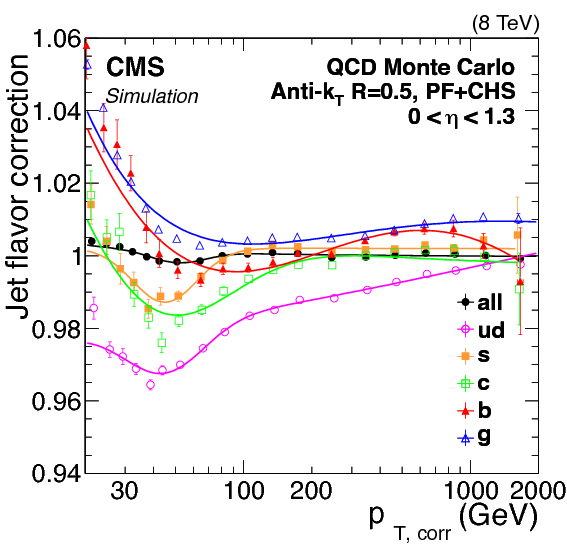
\includegraphics[width=.45\textwidth]{\PhDthesisdir/plots_and_images/from_JERC_RunI/Figure_030-a.png}
\caption[Correction résiduelle de saveur en fonction de l'impulsion du jet.]{Correction résiduelle de saveur en fonction de l'impulsion du jet préalablement corrigée par les corrections décrites dans les sections précédantes, $\pT_\cali$, pour des jets de pseudo-rapidité $\abs{\eta}<\num{1.3}$~\cite{JERC_RunI}.}
\label{fig-chapter-JERC-section-CMS-subsec-PU-JERC_RunI-Figure_030a}
\end{wrapfigure}
Il existe une différence de réponse selon la saveur du jet, majoritairement due à la fragmentation en énergie et la composition du jet qui dépendent de cette saveur~\cite{JERC_RunI}.
Par exemple, les particules de bas \pT\ se retrouvent hors de l'acceptance du détecteur.
Or, des jets initiés par des gluons présentent de nombreuses particules de bas \pT\ par rapport aux jets issus de quarks légers.
Dans une moindre mesure, les jets lourds possèdent également plus de particules de bas \pT\ que les jets de quarks légers suite à la désintégration du hadron lourd.
La proportion de particules neutres dans le jet est également un des paramètres affectant le plus sa réponse.
\par La correction résiduelle de saveur $\mathcal{C}_\text{Sav}$ à appliquer aux données et aux simulations est obtenue à l'aide de
\PYTHIA~6.4~\cite{pythia6.4}
avec les réglages Z2*~\cite{tunes_2016}
sur des événements dijet, \Zjets\ et \Gjets\ simulés
et est représentée sur la figure~\ref{fig-chapter-JERC-section-CMS-subsec-PU-JERC_RunI-Figure_030a}.
Elle est de moins de \SI{2}{\%} en-deçà de \SI{100}{\GeV} mais peut atteindre \SI{4}{\%} à bas \pT.
Dans les analyses de physique des particules, cette correction ne peut être appliquée qu'à condition de connaître la saveur du jet.
Elle n'est donc applicable en pratique qu'aux jets issus de quarks~\quarkb.
\subsection{Incertitude sur la correction en énergie des jets}\label{chapter-JERC-section-CMS-subsec-unc}
Chacune des étapes de la JEC comporte des incertitudes liées aux effets systématiques et, dans une moindre mesure, statistiques.
La maîtrise de ces incertitudes est un enjeu important pour de nombreuses analyses de la collaboration CMS où elles constituent une des sources d'incertitude les plus importantes.
\begin{figure}[p]
\centering
\subcaptionbox{En fonction de $\pT$ pour $\abs{\eta}=0$ en 2016.\label{subfig-Syst_uncs_pT_2016}}[.45\textwidth]
{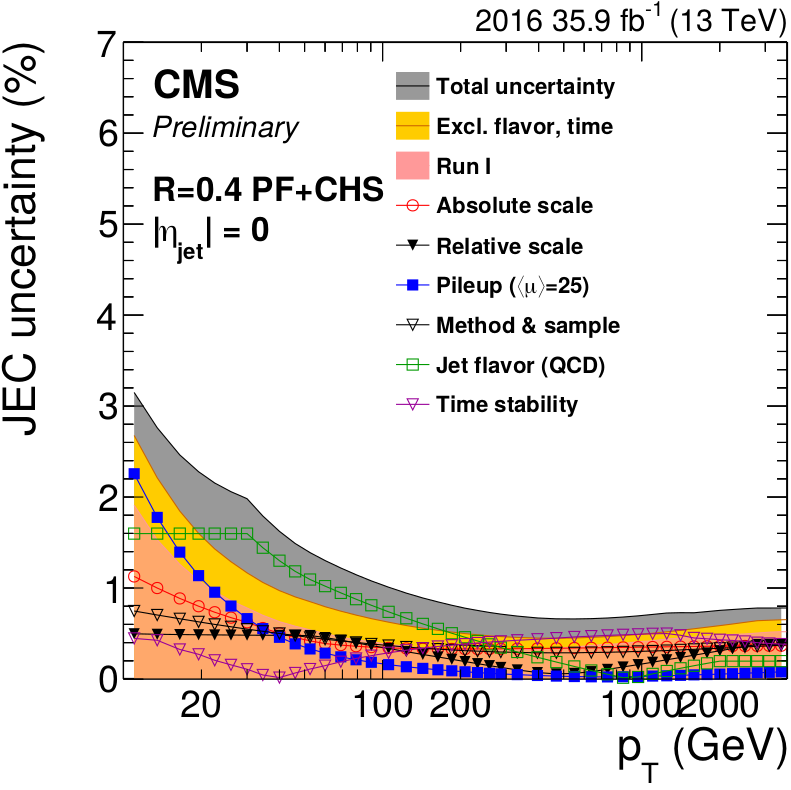
\includegraphics[width=.45\textwidth]{\PhDthesisdir/plots_and_images/from_CMS-DP-2020-019/Syst_uncs_pT_2016.png}\vspace{-.5\baselineskip}}
\hfill
\subcaptionbox{En fonction de $\eta$ pour $\pT=\SI{30}{\GeV}$ en 2016.\label{subfig-Syst_uncs_eta_2016}}[.45\textwidth]
{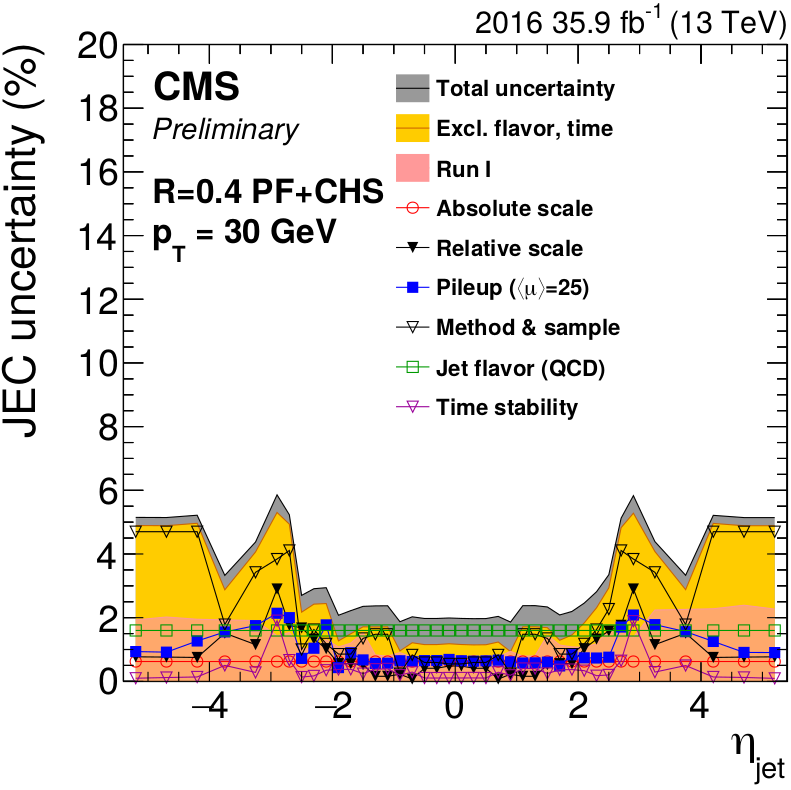
\includegraphics[width=.45\textwidth]{\PhDthesisdir/plots_and_images/from_CMS-DP-2020-019/Syst_uncs_eta_2016.png}\vspace{-.5\baselineskip}}

\vspace{.75\baselineskip}

\subcaptionbox{En fonction de $\pT$ pour $\abs{\eta}=0$ en 2017.\label{subfig-Syst_uncs_pT_2017}}[.45\textwidth]
{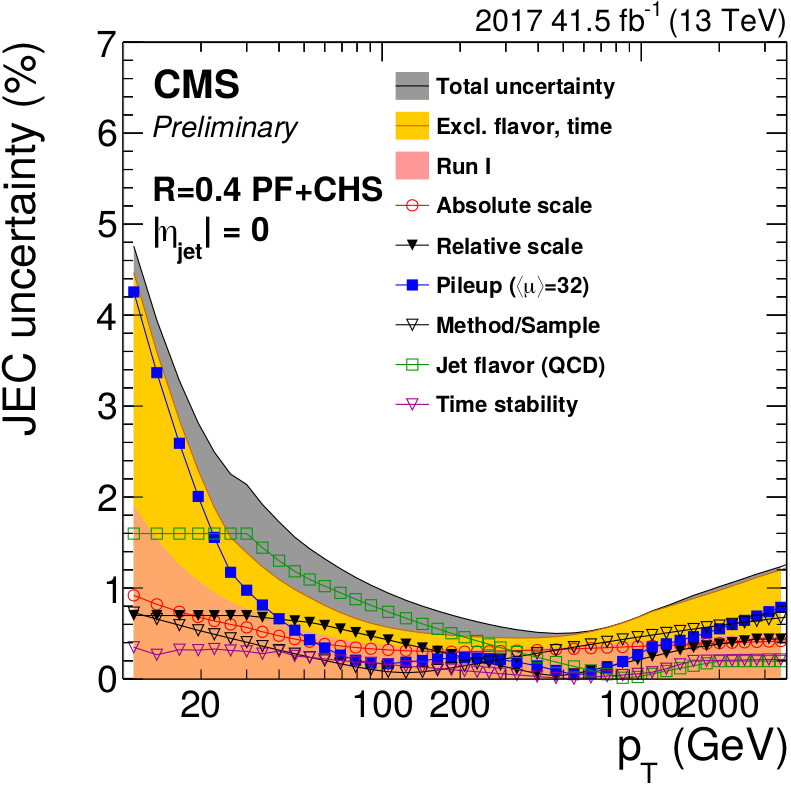
\includegraphics[width=.45\textwidth]{\PhDthesisdir/plots_and_images/from_CMS-DP-2020-019/Syst_uncs_pT_2017.png}\vspace{-.5\baselineskip}}
\hfill
\subcaptionbox{En fonction de $\eta$ pour $\pT=\SI{30}{\GeV}$ en 2017.\label{subfig-Syst_uncs_eta_2017}}[.45\textwidth]
{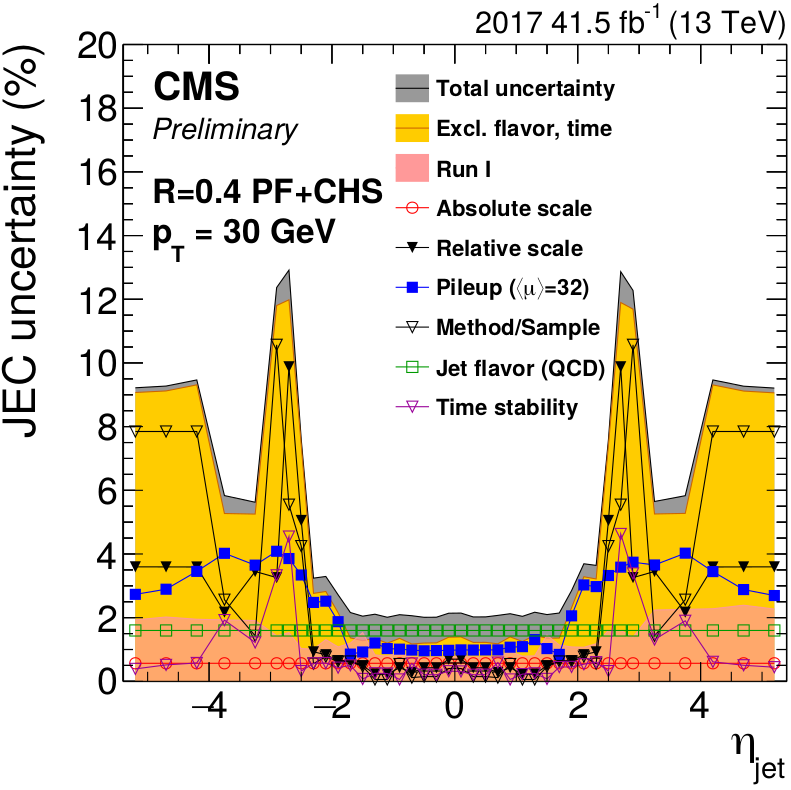
\includegraphics[width=.45\textwidth]{\PhDthesisdir/plots_and_images/from_CMS-DP-2020-019/Syst_uncs_eta_2017.png}\vspace{-.5\baselineskip}}

\vspace{.75\baselineskip}

\subcaptionbox{En fonction de $\pT$ pour $\abs{\eta}=0$ en 2018.\label{subfig-Syst_uncs_pT_2018}}[.45\textwidth]
{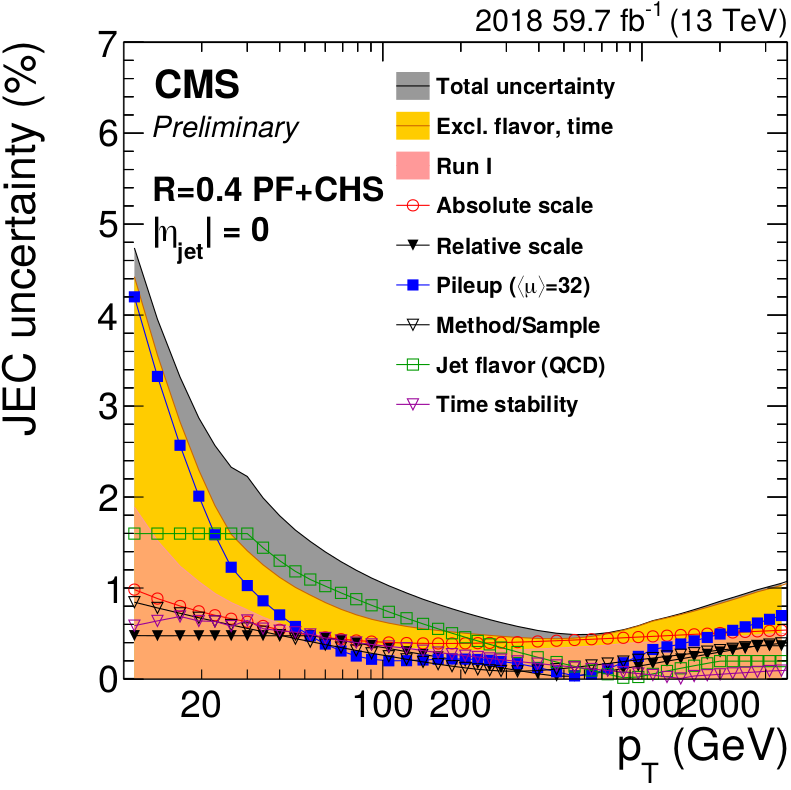
\includegraphics[width=.45\textwidth]{\PhDthesisdir/plots_and_images/from_CMS-DP-2020-019/Syst_uncs_pT_2018.png}\vspace{-.5\baselineskip}}
\hfill
\subcaptionbox{En fonction de $\eta$ pour $\pT=\SI{30}{\GeV}$ en 2018.\label{subfig-Syst_uncs_eta_2018}}[.45\textwidth]
{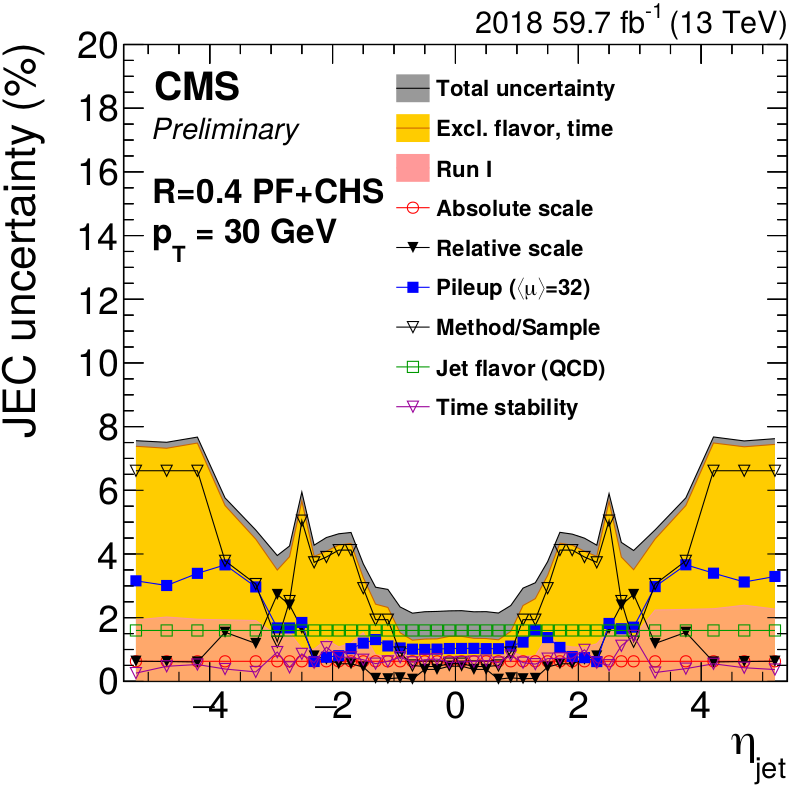
\includegraphics[width=.45\textwidth]{\PhDthesisdir/plots_and_images/from_CMS-DP-2020-019/Syst_uncs_eta_2018.png}\vspace{-.5\baselineskip}}

\caption[Incertitudes relatives sur la JEC en fonction de \pT\ et $\eta$ lors du Run~II.]{Incertitudes relatives sur la JEC lors du Run~II~\cite{CMS-DP-2020-019}.}
\label{fig-Syst_uncs_JEC_RunII}
\end{figure}
Les sources d'incertitude considérées pour la JEC sont réparties en six groupes~\cite{CMS-DP-2020-019}:
\begin{description}
\item[Échelle absolue] ou \emph{Absolute scale} sur les légendes des figures~\ref{subfig-Syst_uncs_pT_2016} à~\ref{subfig-Syst_uncs_eta_2018}.
Cette incertitude prend en compte l'échelle en énergie des objets de référence utilisés pour obtenir la correction résiduelle absolue en \pT\ décrite dans la section~\ref{chapter-JERC-section-CMS-subsec-residuals_pT} ainsi que les effets de l'ISR (\emph{Initial State Radiation}) et du FSR (\emph{Final State Radiation}) abordés dans la section~\ref{chapter-JERC-section-pheno-GJets}.
\item[Échelle relative] ou \emph{Relative scale} sur les légendes des figures~\ref{subfig-Syst_uncs_pT_2016} à~\ref{subfig-Syst_uncs_eta_2018}.
Cette incertitude est principalement due à la JER qui s'applique à l'objet de référence dans la correction résiduelle relative en $\eta$ décrite dans la section~\ref{chapter-JERC-section-CMS-subsec-residuals_eta} ainsi qu'aux effets de l'ISR et du FSR.
\item[Empilement] ou \emph{Pileup} sur les légendes des figures~\ref{subfig-Syst_uncs_pT_2016} à~\ref{subfig-Syst_uncs_eta_2018}.
Il s'agit de rendre compte de l'incertitude sur la détermination de la contribution additionnelle de l'empilement au niveau particule.
Une incertitude de \SI{5}{\%} sur le rapport données sur simulations de cette contribution, obtenue à l'aide de la méthode de cône aléatoire, est considérée.
La différence résiduelle entre la contribution obtenue par cône aléatoire et la contribution réelle extraite des simulations est également prise en compte.
\item[Méthode et jeux de données] ou \emph{Method \& sample} sur les légendes des figures~\ref{subfig-Syst_uncs_pT_2016} à~\ref{subfig-Syst_uncs_eta_2018}.
Cette incertitude correspond aux écarts observés entre les méthodes utilisant les réponses~\Rbal\ et~\RMPF\ d'une part et entre les analyses utilisant les événements \Zjets, \Gjets\ et dijet d'autre part.
\item[Saveur] ou \emph{Jet flavor} sur les légendes des figures~\ref{subfig-Syst_uncs_pT_2016} à~\ref{subfig-Syst_uncs_eta_2018}.
L'incertitude sur la dépendance en saveur de la réponse des jets dans les simulations est estimée à partir de la différence entre deux générateurs,
\PYTHIA~\cite{pythia6.4}
et
\HERWIG~\cite{herwig}.
\item[Stabilité temporelle] ou \emph{Time stability} sur les légendes des figures~\ref{subfig-Syst_uncs_pT_2016} à~\ref{subfig-Syst_uncs_eta_2018}.
La JEC est déterminée pour chaque période de prise de donnée chaque année. Les écarts observés entre ces périodes sont inclus dans cette source d'incertitude.
\end{description}
La figure~\ref{fig-Syst_uncs_JEC_RunII} résume les valeurs de ces incertitudes pour les trois années du Run~II.
L'incertitude globale sur la JEC est généralement inférieure à \SI{2}{\%}, excepté pour les cas $\pT\leq\SI{30}{\GeV}$ ou $\abs{\eta}\geq\num{2}$ où elle peut être de l'ordre de \SI{10}{\%}.
%\subsection{Bilan de la correction en énergie des jets}
%\begin{equation}
%\pT_\cali =
%\underbrace{\underbrace{\underbrace{\pT_\reco^\text{CHS}
%\times
%\mathcal{C}_\text{PU}(\pT_\reco^\text{CHS}, \eta, A, \rho)}_{\pT_\reco'}
%\times
%\mathcal{C}_\text{Rép}(\pT_\reco', \eta)}_{\pT_\reco''}
%\times
%\mathcal{C}_\text{Res}(\pT_\reco'', \eta)}_{\pT_\reco'''}
%\times
%\mathcal{C}_\text{Sav}(\pT_\reco''', \eta)
%\end{equation}
\subsection{Correction de la résolution en énergie}\label{chapter-JERC-section-CMS-subsec-JER}
La résolution en énergie des jets, notée JER, est de l'ordre de \SI{20}{\%} pour des jets à $\pT=\SI{30}{\GeV}$ et de \SI{10}{\%} à $\pT=\SI{100}{\GeV}$~\cite{JERC_RunI}.
Cette résolution est donc bien moins bonne que celles d'autres objets physiques tels que les électrons (\num{2} à \SI{5}{\%}), les muons (\num{1} à \SI{6}{\%}) et les photons (environ \SI{1}{\%}).
La JER joue ainsi un rôle important dans les analyses cherchant des résonances étroites, par exemple.
Il est donc nécessaire de maîtriser cette grandeur.
\par La JER est définie comme la largeur de la gaussienne obtenue par un ajustement sur la distribution de $R_\cali$ des jets, \ie\ $\pT_\cali/\pT_\ptcl$.
Sa mesure est réalisée à l'aide d'événements \Gjets\ et \Zjets\ et les résultats obtenus lors du Run~I sont présentés sur la figure~\ref{subfig-chapter-JERC-section-CMS-subsec-JER-JERC_RunI-Figure_036-b}.
Elle dépend de $\pT_\ptcl$, $\eta$ et $\mu$.
\par La JER observée dans les simulations diffère de celle observée dans les données, elle est légèrement meilleure.
Afin de pouvoir réaliser des analyses comparant données et simulations, il est nécessaire d'avoir une JER comparable dans ces deux catégories d'événements.
La JER des simulations est ainsi détériorée par un facteur d'échelle (JER SF), déterminé à partir d'événements \Gjets\ et dijet et défini en fonction de $\eta$.
Les résultats obtenus lors du Run~II sont présentés sur la figure~\ref{subfig-chapter-JERC-section-CMS-subsec-JER-JER_SF_RunII}.
Le principe est le même que pour les corrections résiduelles décrites dans les sections~\ref{chapter-JERC-section-CMS-subsec-residuals_eta} et~\ref{chapter-JERC-section-CMS-subsec-residuals_pT}. Au lieu de s'intéresser à la moyenne de la distribution, c'est sa largeur qui est étudiée.
\begin{figure}[h]
\centering
\subcaptionbox{JER en fonction de \pT\ dans le barillet de CMS ($\abs{\eta}<\num{1.3}$) pour différentes valeurs d'interactions d'empilement $\mu$ lors du Run~I~\cite{JERC_RunI}.\label{subfig-chapter-JERC-section-CMS-subsec-JER-JERC_RunI-Figure_036-b}}[.45\textwidth]
{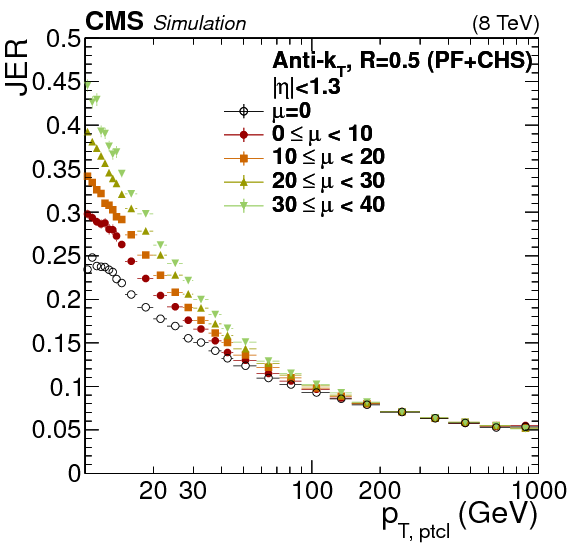
\includegraphics[width=.45\textwidth]{\PhDthesisdir/plots_and_images/from_JERC_RunI/Figure_036-b.png}}
\hfill
\subcaptionbox{Facteurs d'échelle de la résolution en énergie des jets en fonction de $\eta$ lors du Run~II~\cite{CMS-DP-2020-019}.\label{subfig-chapter-JERC-section-CMS-subsec-JER-JER_SF_RunII}}[.45\textwidth]
{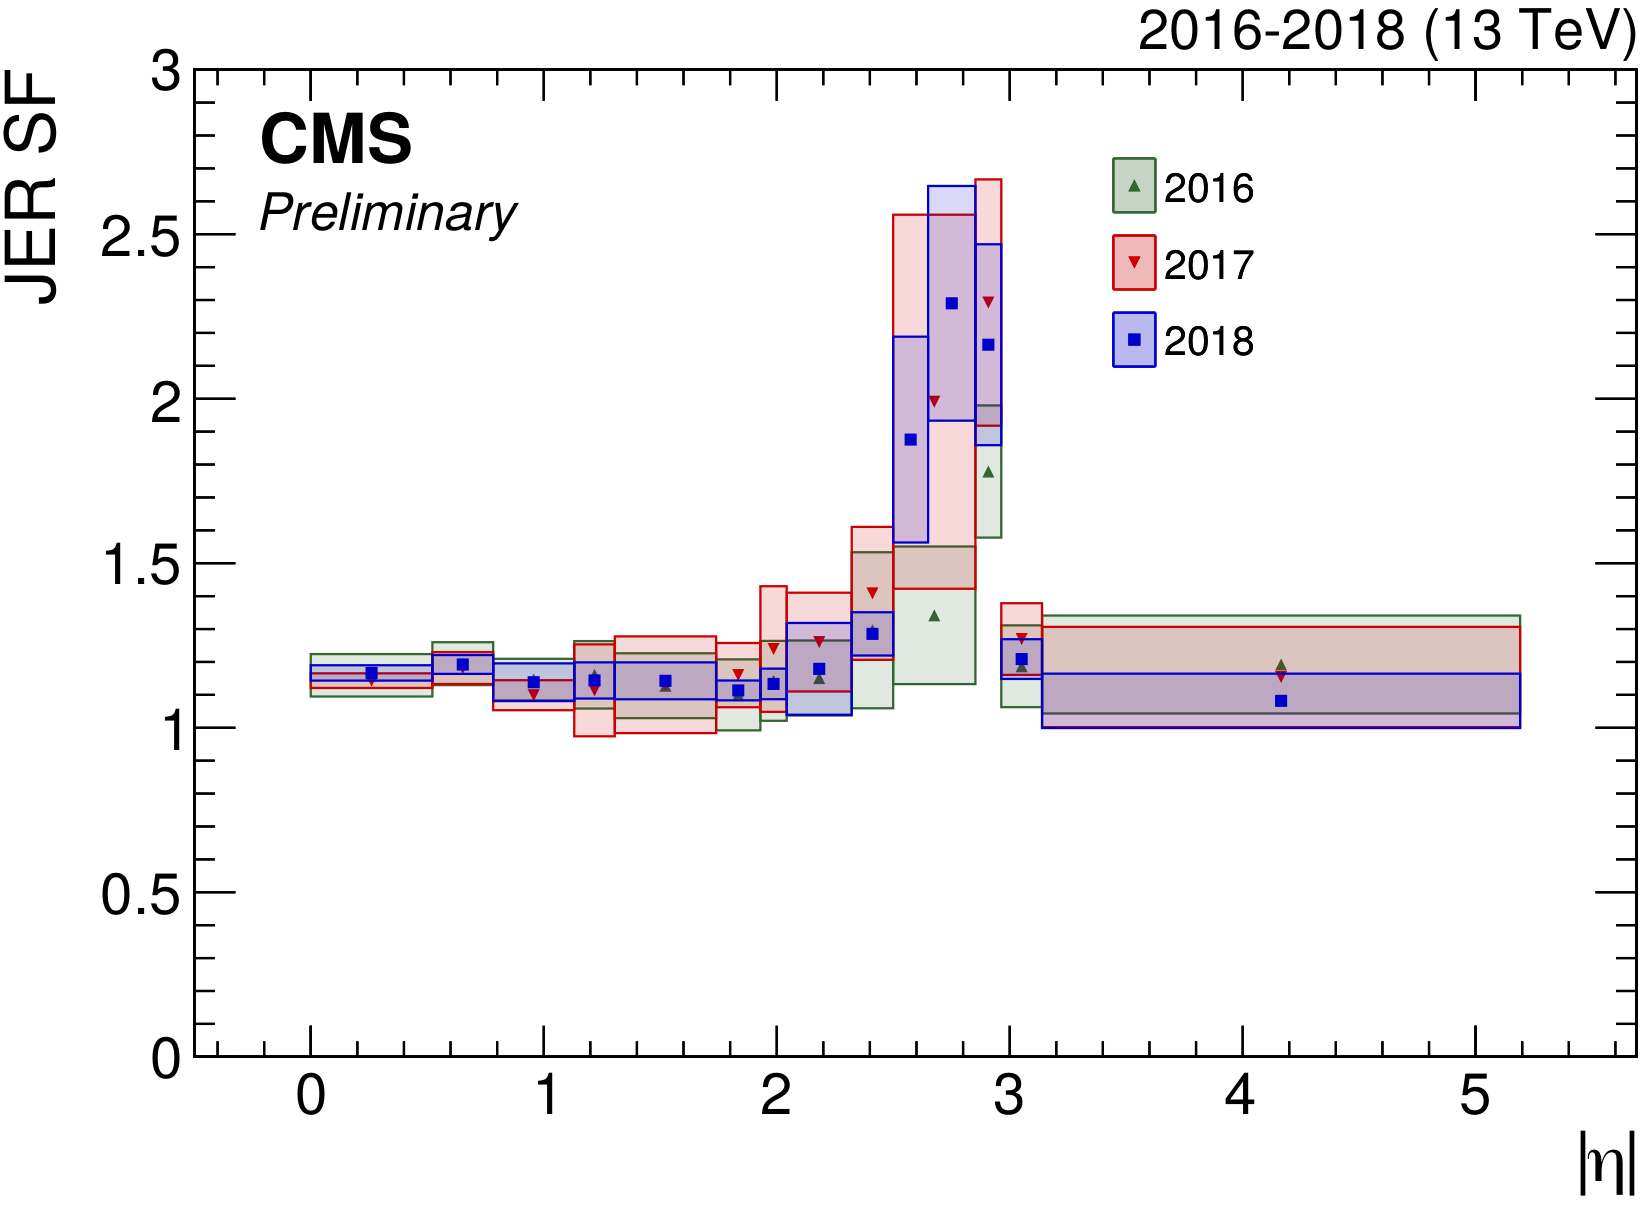
\includegraphics[width=.45\textwidth]{\PhDthesisdir/plots_and_images/from_CMS-DP-2020-019/JER_SF_RunII.png}}
\caption[Résolution en énergie des jets.]{Résolution en énergie des jets dans les simulations et facteurs d'échelle à leur appliquer.}
\label{fig-chapter-JERC-section-CMS-subsec-JER}
\end{figure}
